\chapter{分布式深度学习相关研究}
本章主要介绍分布式深度学习系统涉及的相关技术。从分布式深度学习系统的特点出发,阐述其中设计的难点和重点。从精度和效率两方面分析分布式深度学习系统的特点,并介绍近年来神经网络在不同领域的发展以及目前业界对分布式深度学习的研究进展。
\section{分布式训练神经网络的特点}
随着网络模型的不断增大,数据日益增加以及应用需求的剧增,在深度学习发展历程中,分布式训练神经网络是必不可少的一环。目前主要有数据并行和模型并行两种方法用于分布式训练,如图\ref{fig:data_model_parallel}所示。

\begin{figure}[htp]
\centering
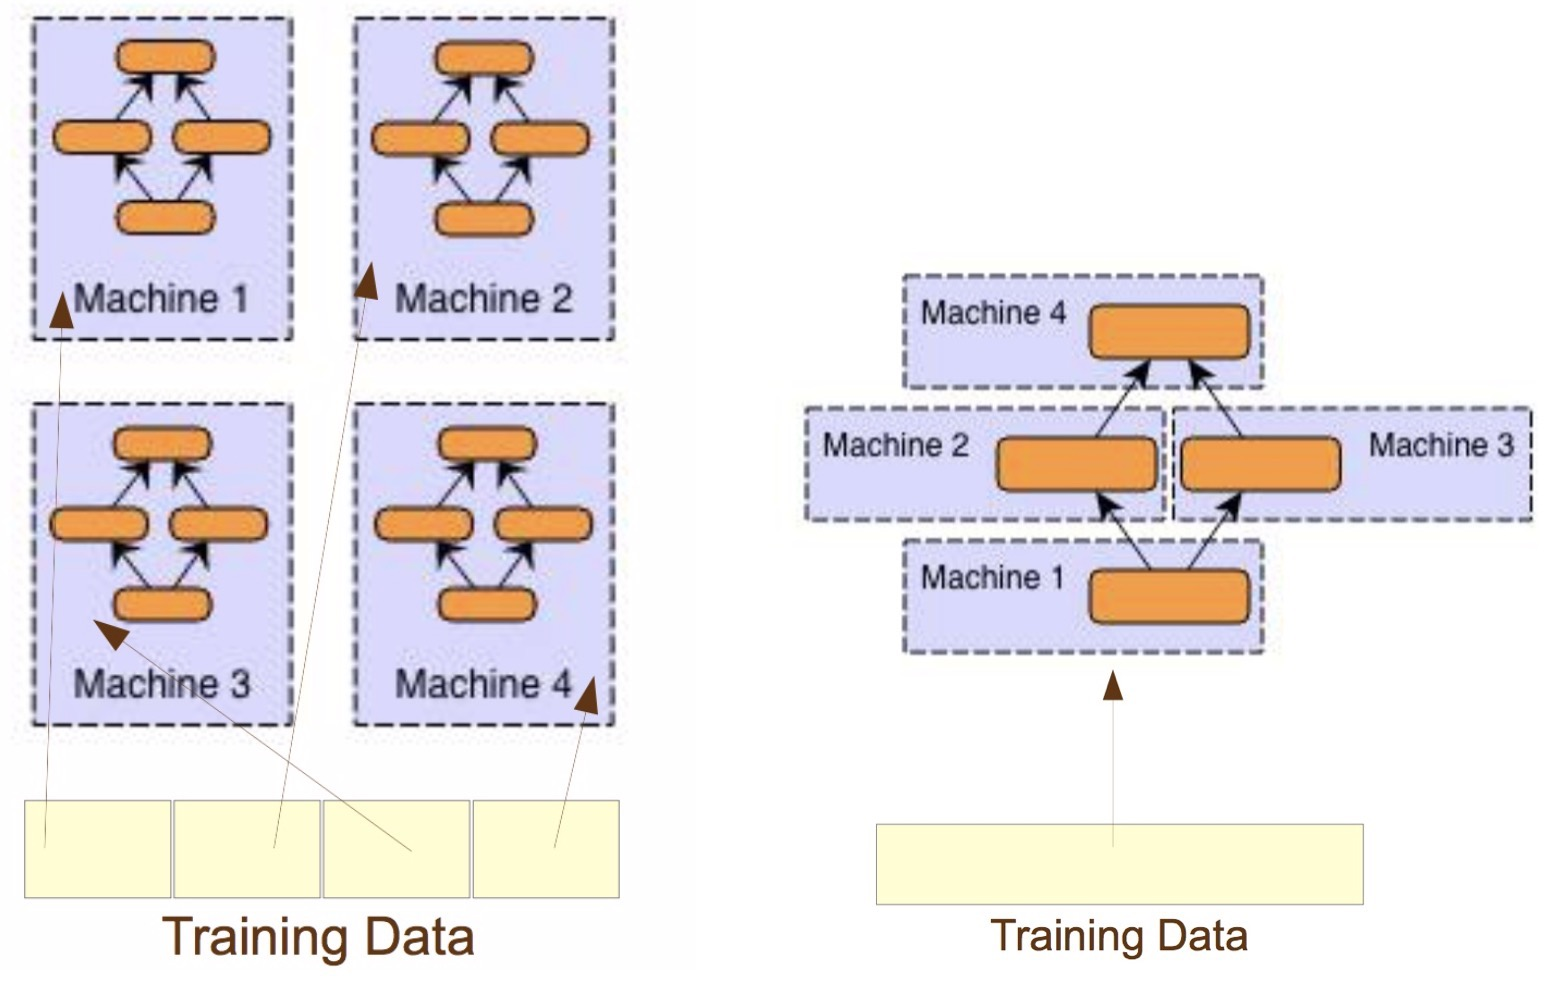
\includegraphics[width=13cm]{data_model_parallel}
\caption{数据并行(左)与模型并行(右)示意图}
\label{fig:data_model_parallel}
\end{figure}
数据并行是把数据分到不同的计算节点上,让不同节点处理不同的数据。因为有多个节点在并行地处理数据,所以在单位时间内,理应能够处理更多的数据,也即达到了并行计算的目的。在数据并行模式下,每个节点都会保留一份完整的网络模型和参数$w^{j}$,在严格同步下,通信主要包含两部分:对本地梯度数据求和,广播全局更新后的参数$w^{j}$到各个节点。在第一步,每个节点都将发送本地梯度$\nabla w^{j}$到管理节点,当管理节点收到所有节点梯度$\nabla w^{j}$时,将对参数进行更新,如公式~\ref{equ:dp_update}所示;第二步管理节点将把全局更新后的$\widetilde w$广播至所有计算节点。
\begin{equation}
\label{equ:dp_update}
\widetilde w \leftarrow \widetilde w - \eta /P \sum^{P}_{j=1}\nabla w^{j}
\end{equation}


模型并行则是把一个大的网络模型划分成很多小块,然后把每小块对应的参数、状态和计算任务分到不同的计算节点上执行,类似于流水线作业。模型并行除通过模型并行获得加速外,当某些模型在单机上无法训练的时候(如内存不够),则只能通过模型并行才能完成训练。目前业界绝大部分训练以数据并行的方式进行训练。

分布式训练神经网络主要有两个指标:一是精度,即随着分布式规模不断增大,在数据并行方法下必然导致用于训练的神经网络的batch size线性增大,即每次迭代更新所用的数据增多,而整体的迭代次数线性降低。当batch size增长到接近数据集大小时,sgd算法就不再适用。在大batch size情况下,如何保证单机batch size一样的精度是分布式深度学习中重要难题。尤其是在分布式规模较大情况下,传统sgd更新算法已经无法保证训练精度,需要新的更新算法保证网络精度。
如facebook提出的热启动、线性增大学习率方法\upcite{train1hour2017},在保证训练精度情况下,将batch size提升至8k;线性增大学习率是指:当batch size从$B$增大到$kB$时,此时学习率也要由$\eta$增大至$k\eta$;热启动则表示:学习率$\eta$应逐渐增大至$k\eta$,假设热启动的迭代次数为$I$,则在第$i$次迭代中学习率为$\eta _{i}=\eta + i(k-1)\eta/I$。
随后用伯克利的尤洋等\upcite{train24min2017}提出的分层自适应学习率的方法,进一步将batch size提升至32k;其核心思想是每个网络层参数及其梯度数值差距很大,不应使用相同学习率$\gamma$对其进行更新,而应设置不同学习率分别更新对应参数。其学习率计算如公式~\ref{equ:lars}所示。
\begin{equation}
\eta = l \times \gamma \times \frac{||w||_{2}}{||\nabla w||_{2}}
\label{equ:lars}
\end{equation}

进一步谷歌大脑\upcite{dontdecay2018}提出通过逐渐增大batch size替换学习率衰减的方法,最终将batch size提升至64k,只用两千五百多次迭代将ImageNet训到了理想精度。二是效率,即在保证精度的情况下,训练系统的效率要尽可能高,分布式相对于单节点的加速比越接近理想加速比则系统可扩展性越好。而根据分布式训练更新特点可知,分布式训练相对于单机训练区别在于多了同步全局梯度的开销,计算开销与单机相同。故同步梯度开销的大小对分布式深度学习系统的训练效率和可扩展性好坏至关重要。

为减少同步梯度的开销,涌现出了一系列异步,半异步的方法,如Hogwild\upcite{hogwild2011}提出lock free方法,在稀疏问题上具有显著效果;Sixin Zhang等人提出弹性均值随机梯度下降算法\upcite{easgd2015},通过预估节点梯度与全局梯度的差值来弥补异步更新的不足,达到理想效果;Peter等\upcite{scaledist2016}提出gossiping sgd算法,类似于去中心化的EASGD算法,在节点规模较小的情况下,收敛速度快于传统sgd算法;随后,Ioannis Mitliagkas等\upcite{asynmomentum2016}提出一种新颖的momentum更新方法,将节点梯度与全局梯度的差距当成隐含的momentum来解释,从而提出通过设置反向momentum的方法抵消局部梯度与全局梯度之间的差异。

目前神经网络的训练基本是用sgd算法或sgd算法的变种。在分布式训练神经网络中,异步或半异步的sgd算法无法达到正常收敛水平,能够保证神经网络收敛精度的异步或半异步的更新算法有待科学家进一步研究探索。目前分布式训练神经网络主要采用严格同步的更新方法,这使得提高训练系统效率更为困难。
\section{神经网络的发展}
近年来神经网络因其突出的性能在各个领域得到广泛应用。下面分别从图像分类、物体检测、自然语言处理三个领域对神经网络发展的进行介绍。
\subsection{神经网络在图像分类领域的发展}
AlexNet\upcite{alexnet2012},将卷积神经网络用于图像分类的开山之作。2012年在ImageNet上刷新各项纪录,夺得冠军,掀起一股神经网络热潮。其网络结构如图~\ref{fig:AlexNet}所示。受当时设备算力和显存的影响,作者将模型放在两块GPU上共同训练,网络总共8层。最终以超过第二名8.2\%的分数夺得冠军。

\begin{figure}[htp]
\centering
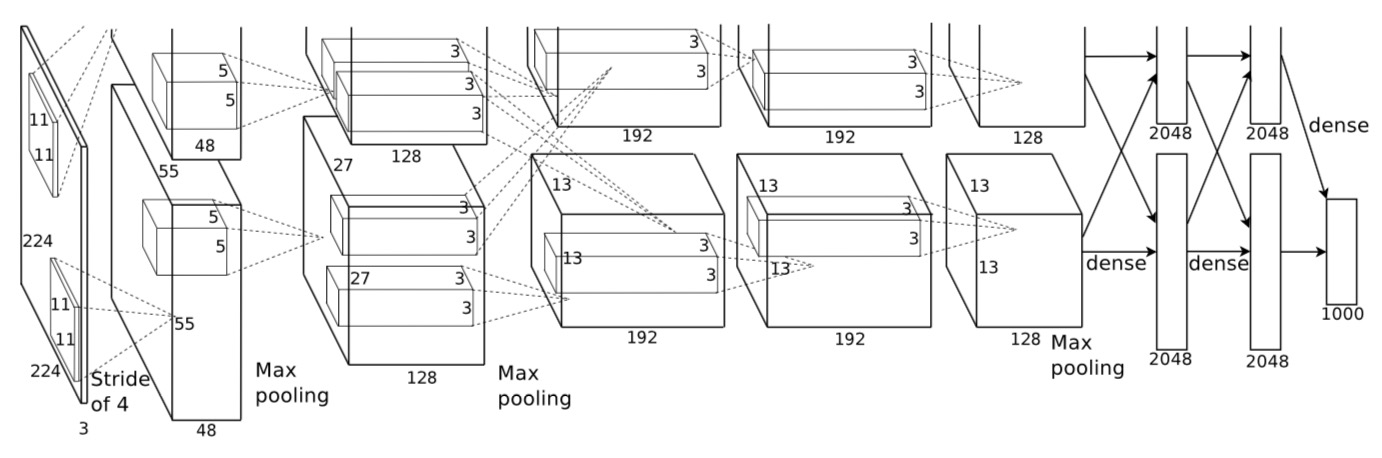
\includegraphics[width=13cm]{AlexNet}
\caption{AlexNet网络结构示意图}
\label{fig:AlexNet}
\end{figure}
随后,DeepMind提出了性能更强网络结构更深的VGG\upcite{vgg2014}系列网络。同时相对于AlexNet,该网络结构也更加规则化,为神经网络提供了一个模块化设计的思路,为以后设计更大更深的网络提供思路。此后基于卷积神经网络的各种基本组件,就可以像搭积木一样设计出相应的网络结构。

同时,google也提出性能更强,类似网中网的网络结构Inception\upcite{inception2015}系列。即网络的基本组件不再是简单的单层结构。而是偏复杂的module结构,类似一个小型的网络模块,如图~\ref{fig:inception_picture}所示。

\begin{figure}[htp]
\centering
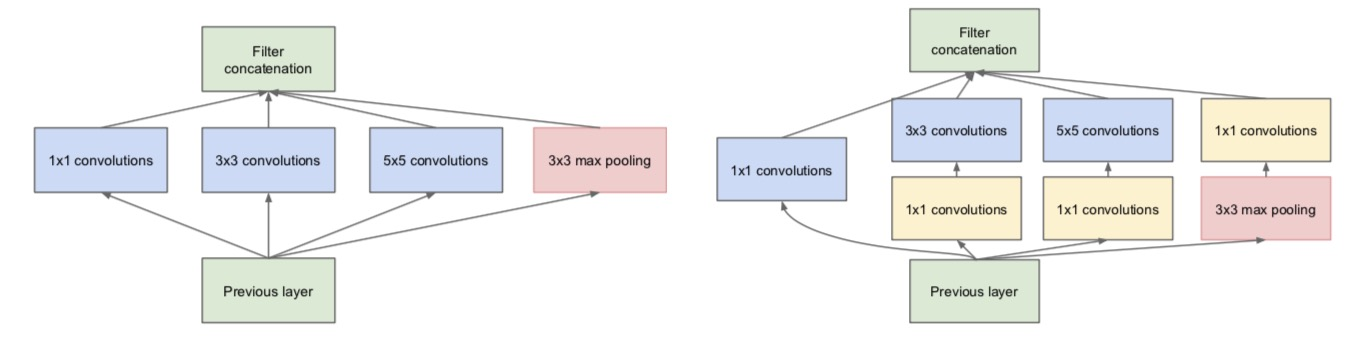
\includegraphics[width=12cm]{inception_picture}
\caption{inception module结构示意图}
\label{fig:inception_picture}
\end{figure}
如图~\ref{fig:inception_picture}分别展示了下采样和不下采样情况下,module的结构模型。随后基于inception提出了一系列的改进版如inception-V2,inception-V4等。从中可以看出网络设计越来越趋向于结构化。卷积核的形状也越来越规整,基本以3x3卷积为主,没有了诸多不同尺寸的卷积核设计。

随后,Kaiming He等\upcite{resnet2016}提出声名大噪的ResNet,一举夺得CVPR 2016年最佳学术论文奖。其计算量、参数量远小于VGG,inception,而精度则比其他网络要高。其核心思想来源于传统机器学习中的残差学习。提出让逐层网络学习上一层网络的残差,比直接学习特征要相对容易。基本残差结构如图~\ref{fig:resnet_block}所示。

\begin{figure}[htp]
\centering
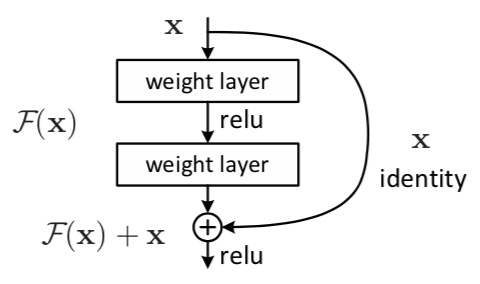
\includegraphics[width=10cm]{resnet_block}
\caption{ResNet block结构示意图}
\label{fig:resnet_block}
\end{figure}
2017年,Gao Huang等\upcite{denselynet2017}基于残差连接的思想,提出DenseNet。其核心思想是为了使后层网络获取前部分网络尽可能多的信息。使其分别与前面各层建立连接,从而形成相对密集连接的DensetNet网络,如图~\ref{fig:DenseNet_picture}所示。

\begin{figure}[htp]
\centering
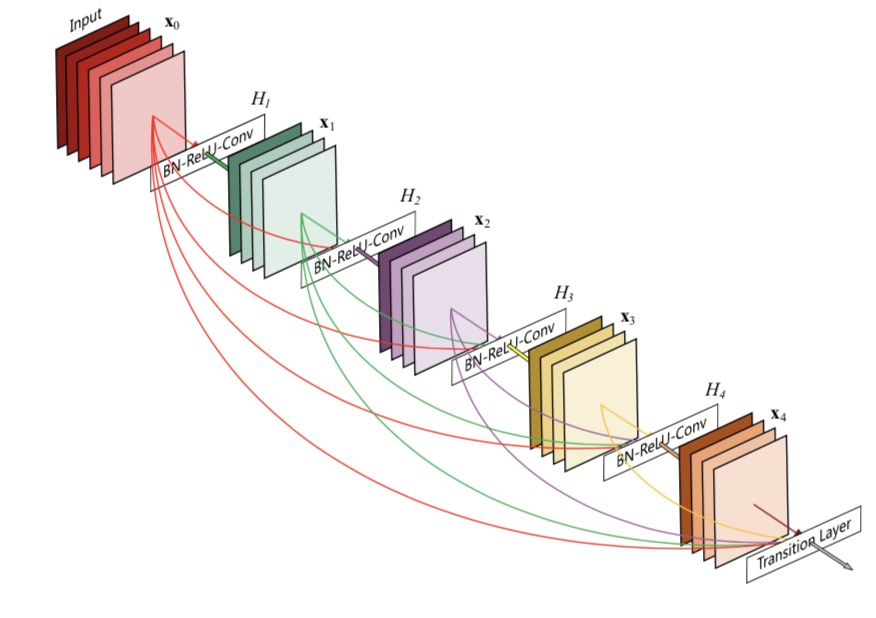
\includegraphics[width=12cm]{DenseNet_picture}
\caption{DenseNet结构示意图}
\label{fig:DenseNet_picture}
\end{figure}
随着越来越多的神经网络部署到实际应用中,其对网络计算量提出了许多限制要求。因为在算力受限的设备中如:手机,个人电脑以及其他嵌入式设备等,无法对计算量大的网络完成计算,或计算量过大则无法满足其实时性要求。受限算力下的小型网络结构应运而生。

2017年,Andrew G. Howard等\upcite{mobilenet2017}提出轻量级网络MobileNet。其核心思想是根据传统卷积的作用:扩大感受野和融合通道间的特征。分别用计算量偏小的depthwise convolution和pointwise convolution代替,极大减少了网络的计算量,其替换原理图如图~\ref{fig:mobilenet}所示。在相同计算量的情况下,达到了非常好的性能。

\begin{figure}[htp]
\centering
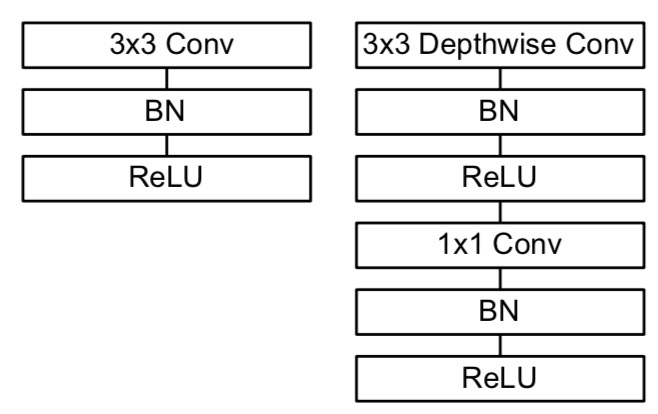
\includegraphics[width=12cm]{mobilenet}
\caption{传统conv+BN+Relu(左)与depthwise separable conv(右)示意图}
\label{fig:mobilenet}
\end{figure}
随后,Xiangyu Zhang等\upcite{shufflenet2018}提出ShuffleNet,进一步减小了网络计算量。在相同计算量情况下,网络性能达到最好情况。其核心思想是把pointwise convolution进行分组,根据卷积计算公式可知,分组越多,计算量越少,通道间信息传递也越少。为了使通道间信息能更好的融合,论文提出shuffle的方式将各层通道的信息进行融合,示意图如图~\ref{fig:shufflenet}所示。其主要包含两个步骤:一是对pointwise做分组卷积;二是对分组后的卷积在通道之间做shuffle,以保证通道间的信息融合。

\begin{figure}[htp]
\centering
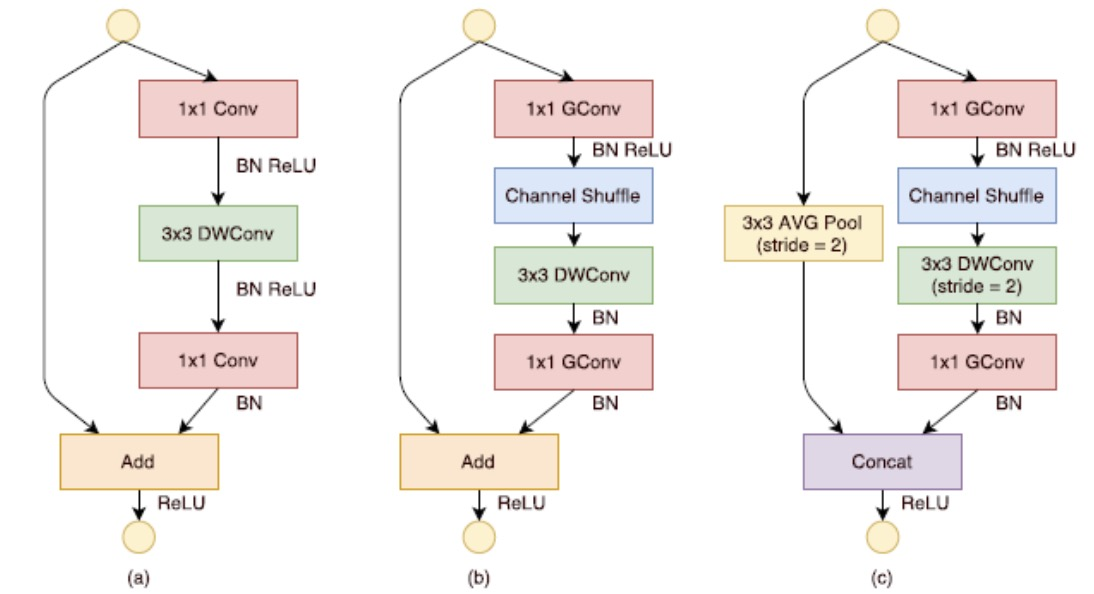
\includegraphics[width=14cm]{shufflenet}
\caption{bottleneck单元(a)组卷积单元(b)stride=2的组卷积单元(c)示意图}
\label{fig:shufflenet}
\end{figure}
\subsection{神经网络在物体检测领域的发展}
随着神经网络在图像分类领域取得的显著进展,人们开始将卷积神经网络应用于物体检测领域。近年来卷积神经网络在该领域也取得了突飞猛进的发展。目前基于神经网络的检测算法主要分为两种:一阶段检测网络和二阶段检测网络。一阶段网络速度较快,精度偏低;二阶段网络速度偏慢,精度较高。下面分别介绍一阶段网络和二阶段网络中相关的研究进展。

2014年,Ross Girshick等\upcite{rcnn2014}提出的R-CNN网络是将神经网络用于目标检测领域的开山之作。其主要分为三个步骤:1.用传统方法selective-search从原始图片中选取出2k个框;2. 将这些框对应的图片送入卷积神经网络,提取对应框的特征;3.使用传统SVM分类器对得到的特征进行分类。其算法流程图如图~\ref{fig:rcnn_overview}所示。

\begin{figure}[htp]
\centering
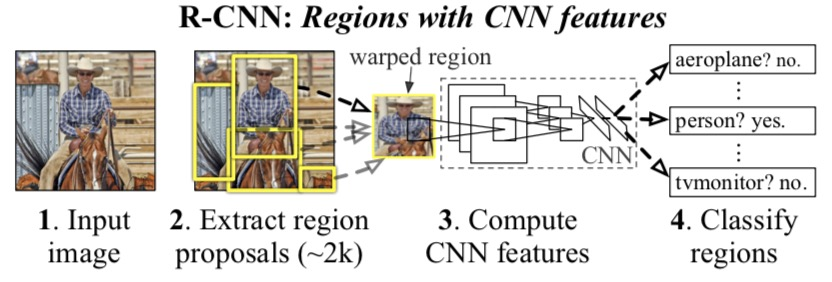
\includegraphics[width=12cm]{rcnn_overview}
\caption{R-CNN算法流程图}
\label{fig:rcnn_overview}
\end{figure}
由其算法流程图可知,该算法流程耗时较复杂。因为一张图片同时提取2k个框,提取的特征数据量巨大,占用磁盘空间较大,如5000张图片会产生几百G的特征文件,且因为一张图片中的每个特征框都得过一遍神经网络,其处理速度非常慢,平均47秒处理一张图片。

针对R-CNN训练速度慢的问题,2015年Kaiming He等\upcite{sppnet2014}提出SPPNet。其分析了R-CNN之所以速度慢的原因在于一张图片要过2k次神经网络。根本原因在于不同框的尺寸不同,而网络最后的分类部分要求特征图尺寸一致,这种矛盾使得2k个框只能分别输入神经网络。为克服这个问题,论文提出空间金字塔池化方法,其结构示意如图~\ref{fig:sppnet}所示。通过该方法将不同尺寸的特征图池化到相同尺寸,从而使得一张图片只需过一遍神经网络,极大提升了网络性能。

\begin{figure}[htp]
\centering
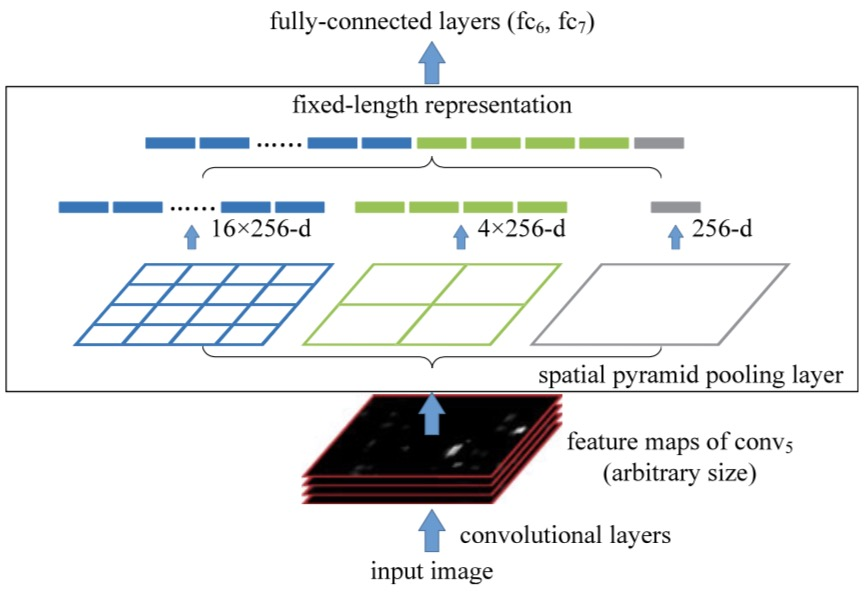
\includegraphics[width=10cm]{sppnet}
\caption{SPP结构示意图}
\label{fig:sppnet}
\end{figure}
随后,Ross Girshick根据R-CNN的缺点,以及SPPNet的优点,提出Fast R-CNN\upcite{fastrcnn2015},主要有两个工作:1.将R-CNN中SVM的分类部分用卷积神经网络代替;2.改进SPP的池化方法,提出ROI pooling方法。Fast R-CNN的网络结构如图~\ref{fig:fast_rcnn}所示。

\begin{figure}[htp]
\centering
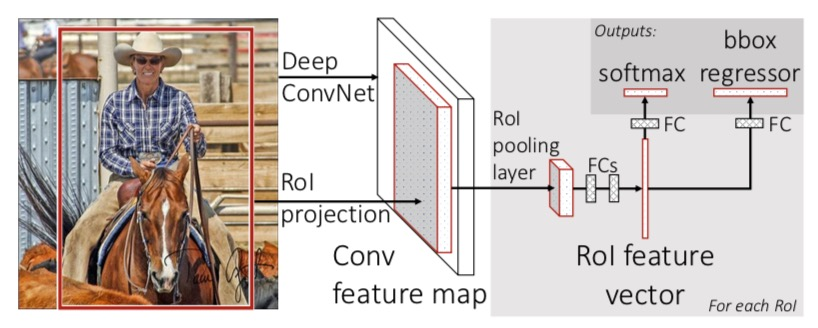
\includegraphics[width=10cm]{fast_rcnn}
\caption{Fast R-CNN算法流程图}
\label{fig:fast_rcnn}
\end{figure}
基于Fast R-CNN的工作,Shaoqing Ren, Kaiming He和Ross Girshick进一步提出Faster R-CNN\upcite{fasterrcnn2015}检测网络。为了解决Fast R-CNN网络提取框耗时的问题,论文提出用于提取检测框的FPN网络,进一步提升了训练速度,实现了真正意义上的端到端训练。FPN网络结构如图~\ref{fig:fpn}所示。随后也出现了各种网络如:R-FCN\upcite{rfcn2016},focal loss\upcite{focalloss2017}等。

\begin{figure}[htp]
\centering
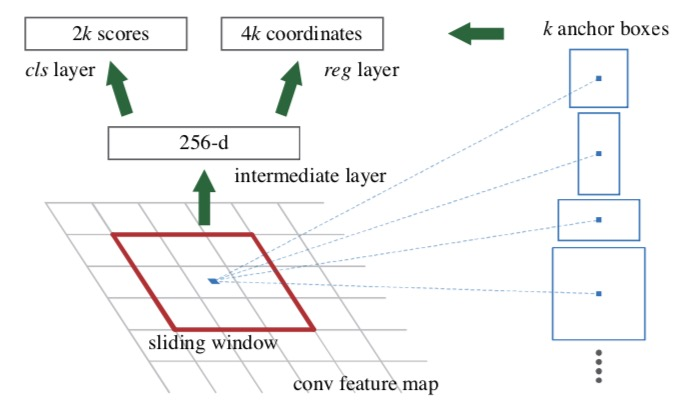
\includegraphics[width=10cm]{fpn}
\caption{FPN网络结构图}
\label{fig:fpn}
\end{figure}
另一方面,一阶段目标检测网络也发展迅猛。2016年,Joseph Redmon等提出yolo网络\upcite{yolo2016},其核心思想是直接让网络预测出每个特征点的类别和对应框的4个坐标。其网络结构如图~\ref{fig:yolo}所示。因其检测速度快的优势,得到广泛使用,随后基于yolo不断进行改进,yolo2,yolo3也相继发表提出。

\begin{figure}[htp]
\centering
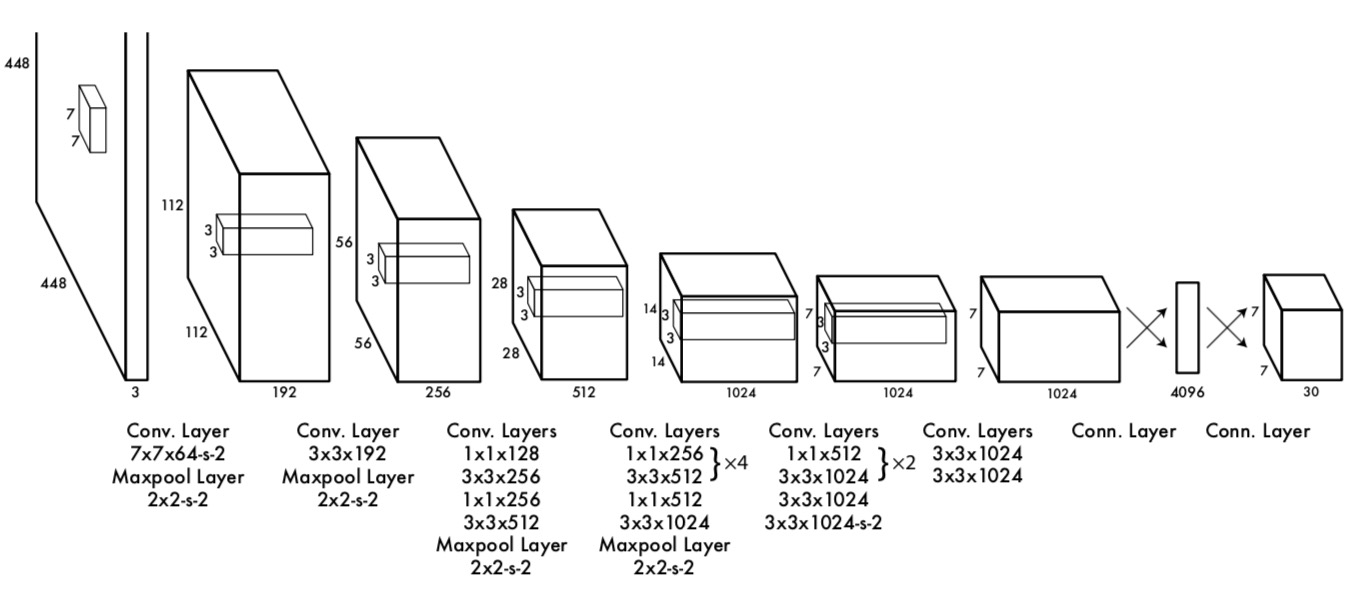
\includegraphics[width=14cm]{yolo}
\caption{yolo网络结构图}
\label{fig:yolo}
\end{figure}
同年Wei Liu等提出SSD网络\upcite{ssd2016},结合了Faster R-CNN和yolo的优点,采用了Faster R-CNN的anchors机制,同时是和yolo相同的一阶段检测方法。网络结构如图~\ref{fig:ssd}所示。其使用不同层的feature map预测不同的大小的框,不同层的feature map可以预测不同大小的物体,达到预测不同大小物体的目的。

\begin{figure}[htp]
\centering
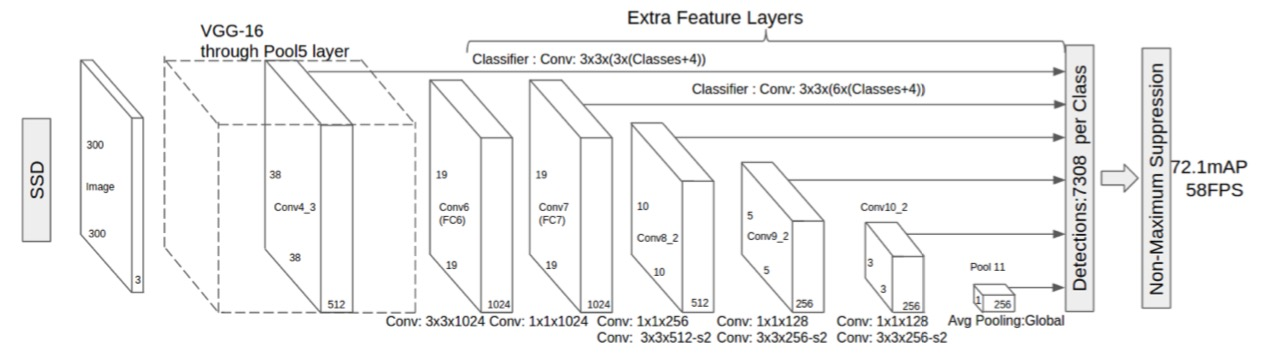
\includegraphics[width=14cm]{ssd}
\caption{ssd网络结构图}
\label{fig:ssd}
\end{figure}
\subsection{神经网络在自然语言处理领域的发展}
在自然语言处理领域,神经网络被用在了机器翻译,文本处理,阅读理解等诸多方面。2016年,谷歌提出其机器翻译模型GNTMT\upcite{gnmt2016}。其引入了注意力机制使得系统处理长句子时更准确高效。针对神经网络系统的三个弱点:1.训练速度很慢并且需要巨大的计算资源。由于参数量计算量过大,其翻译速度也远低于传统的基于短语的翻译系统;2.对罕见词的处理很无力,传统神经网络直接复制原词的方式在很多情况下不是一个好的解决方法;3.在处理长句子的时候会有漏翻译的现象。GNMT使用了8层含有残差连接的循环神经网络,其结构如图~\ref{fig:gnmt}所示。残差连接可以帮助某些信息的传递,比如梯度、位置信息。同时,attention层与decoder的底层以及encoder的顶层相连接。

\begin{figure}[htp]
\centering
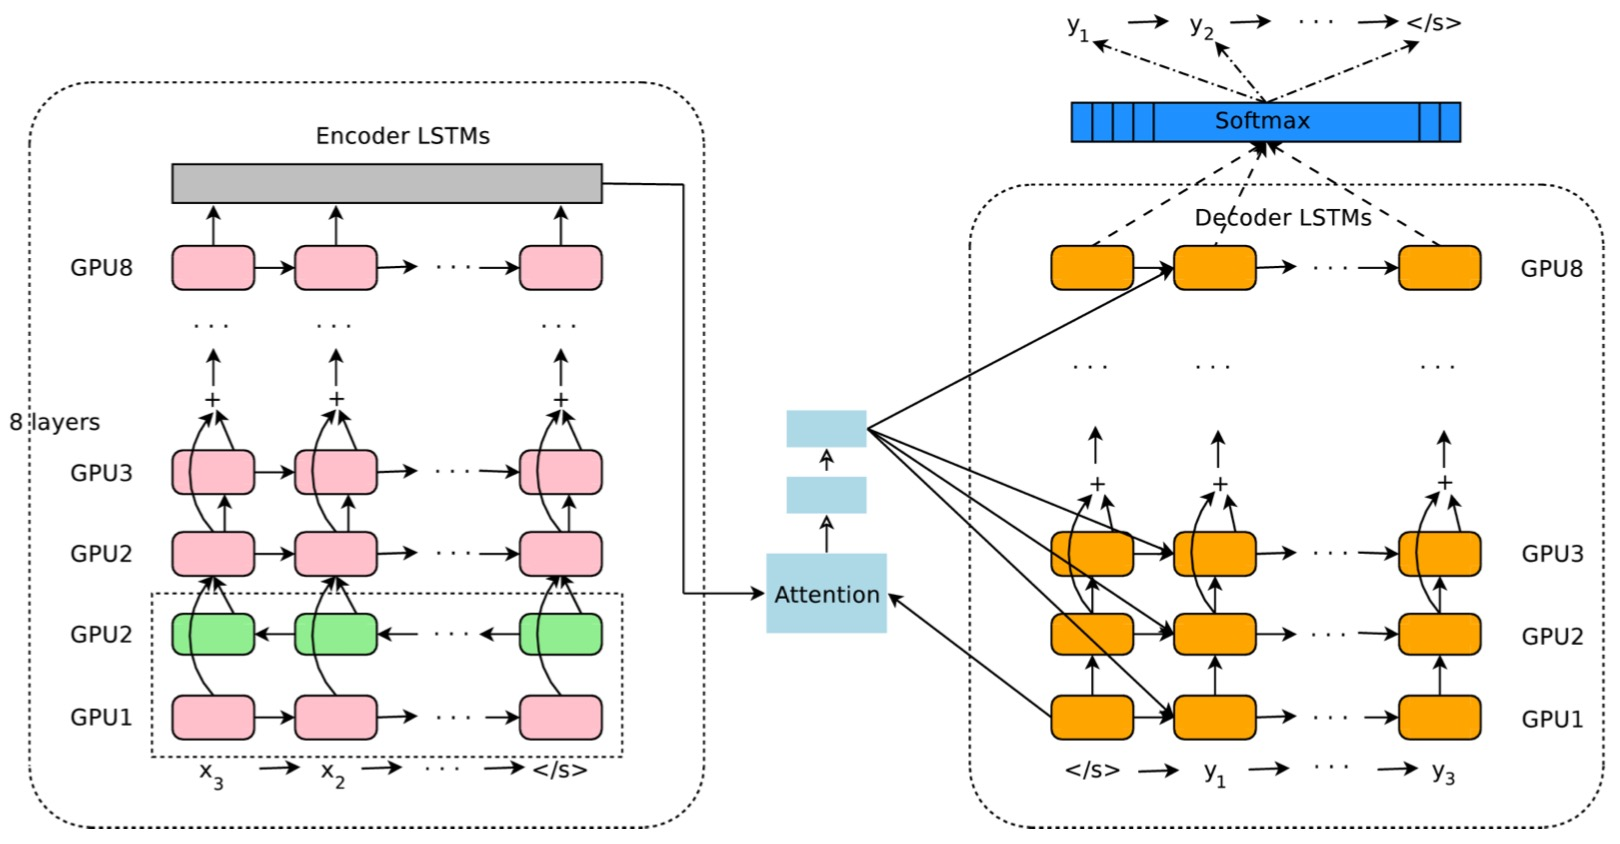
\includegraphics[width=14cm]{gnmt}
\caption{gnmt网络结构图}
\label{fig:gnmt}
\end{figure}
2018年,谷歌提出BERT\upcite{bert2018}模型,刷新了多项NLP任务的成绩,是一项里程碑式的工作。使用了masked lm和下一句预测的联合训练方法,在加上12层的transformer。
\section{分布式深度学习的发展}
分布式深度学习涉及到的领域很广。涵盖优化算法、模型、系统和应用等。下面分别介绍以下三个方向的研究进展:分布式系统、优化算法和数据压缩。
\subsection{分布式深度学习系统的发展}
自2012年底AlexNet\upcite{alexnet2012}在ImageNet上大放异彩,刷新诸多记录,从此开启了深度学习的新篇章。同年,对应的分布式深度学习系统也应运而生。Jeffrey Dean等提出的DistBelief\upcite{distbelief2012},即Google的第一代深度学习系统,其核心实现是把分布式机器学习里面的数据并行(data parallelism)和模型并行(model parallelism)用在深度学习上,通过这两种并行方法把深度学习大规模部署到集群。同时,论文提出了分布式异步SGD—DownPour SGD和L-BFGS算法,在CPU集群上系统效果显著。

随后,考虑到分布式训练网络过程中的同步通信开销,Qirong Ho等\upcite{ssp2013}提出了松弛一致性模型:Stale Synchronous Parallel(SSP), 如图~\ref{fig:ssp_picture}所示。解决了严格同步(BSP)模型下木桶效应导致同步时间过长的问题,提高了计算效率。并基于该模型,搭建了Petuum系统。

\begin{figure}[htp]
\centering
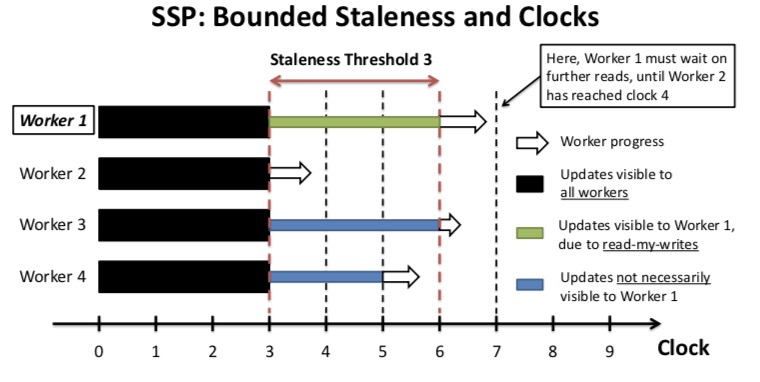
\includegraphics[width=12cm]{ssp_picture}
\caption{SSP模型示意图}
\label{fig:ssp_picture}
\end{figure}
同时期,Adam Coates等\upcite{cots2013}搭建了一个GPU集群:COTS HPC system,该系统通过模型并行方法分布式训练网络模型。因为该系统使用GPU计算,CPU用于通信。在InfiniBand 50 Gb网络上测试,计算在毫秒级完成,而通信时间则需要8秒,系统效率极差,为克服通信瓶颈,其提出一种复杂有效的GPU协作算法,进一步了提升集群效率。

紧接着Microsoft推出了基于参数服务器的深度学习系统Adam\upcite{adam2014}。其是一个CPU集群,通过模型并行的方式训练神经网络。为避免数据处理速度跟不上,系统专门用四台机器用于数据预处理,并将模型放在L3 cache上。为了提升网络间数据的传输性能,该系统设计了一种专门的网络IO,避免不必要的数据拷贝、传输。

分布式深度学习中一个关键的通信组件是参数服务器(Parameter Server),最早由Alex Smola提出,因其简单、高效的特点,被广泛用于分布式深度学习进行参数同步。最著名的参数服务器框架要数李沐等人做的Parameter Servers\upcite{ps2014},并进一步开发出MXNet。在李沐等人的Parameter Servers框架中,其集成了传统分布式框架Hadoop、Spark的优点,通过图遍历、消息压缩和去中心化等优化方法,理论性能与allreduce一致,实际性能十分优异,但其对CPU需求较大,当CPU承担任务过多时,容易因为竞争冲突导致性能下降。

随后,Henggang Cui等\upcite{geeps2016}在GPU上实现了Parameter Servers,推出GeePS系统,避免了CPU通信过程中GPU与CPU之间的数据拷贝,提高了数据通信效率。同时为缓解模型占用GPU显存过多的问题,提出一种GPU内存管理机制,使得在GPU受限情况下,训练更大的网络成为可能。
\subsection{分布式深度学习中优化算法的发展}
在分布式深度学习系统中主要分为异步算法和同步算法。下面分别介绍分布式深度学习中近年来异步和同步算法的研究进展。

2011年,Feng Niu等\upcite{hogwild2011}针对稀疏求解问题,提出异步更新方法即lock-free方法。因为是稀疏问题,每个worker需要更新的参数几乎均不一样,重叠率很低。所以不用以严格顺序更新,异步更新即可。2014年,Henggang Cui等\upcite{absp2014}提出一种结合ssp和wpc-bsp的算法A-BSP。算法原理图如图~\ref{fig:a_bsp}所示。大致内容为:在bsp中每次迭代都同步更新梯度,使得同步等待的时间在总体训练时间过长。为了减少同步等待的时间比重,提出每间隔wpc次迭代才同步更新一次,减少同步等待时间占整体时间的比重。该算法每隔$n$个迭代才同步更新一次,等效于增大batch size。但与之不同的是在$n$个迭代之间各个worker会根据本地的参数更新。

\begin{figure}[htp]
\centering
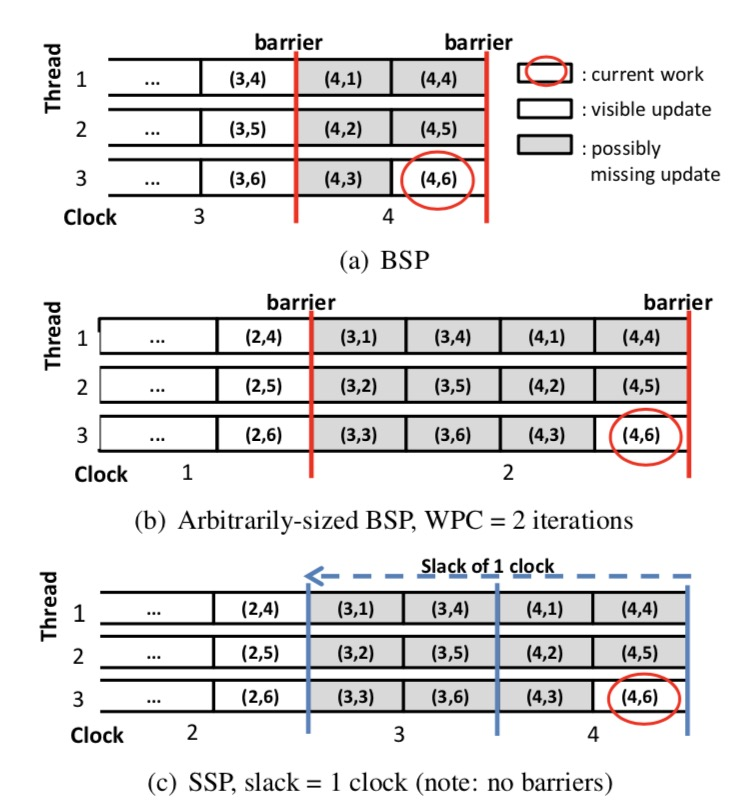
\includegraphics[width=12cm]{a_bsp}
\caption{bsp,a-bsp,ssp示意图}
\label{fig:a_bsp}
\end{figure}
2015年,Sixin Zhang等\upcite{easgd2015}提出异步的弹性均值sgd算法。其设计思想为:每个worker进行参数更新时,除了要考虑当前梯度,还应考虑当前worker的参数与中心节点master的全局参数的差距。不仅要减去当前worker的梯度,还应该减去这个差值。在第$t$次迭代中,以学习率$\eta$对优化目标$g$中的参数$x$进行更新时,worker和master节点更新如公式~\ref{equ:easgd_worker},~\ref{equ:easgd_master}所示,其中$\rho$类似于动量。
\begin{equation}
\label{equ:easgd_worker}
x^{i}_{t+1}=x^i_t-\eta(g^i_t(x^i_t)+\rho(x^i_t-\widetilde x))
\end{equation}
\begin{equation}
\label{equ:easgd_master}
\widetilde x_{t+1}=\widetilde x_t +\eta \sum_{i=1}^{p}\rho(x^i_t - \widetilde x_t)
\end{equation}

随后,2016年Peter H等基于EASGD算法提出gossiping算法\upcite{scaledist2016}。与EASGD算法相似,是一个去中心化的EASGD算法,其将中心节点更新的全局参数直接用各worker参数的均值代替了。该论文实验结果有诸多启发性的结论:1. 在小节点情况下(节点数在32个以内),异步的EASGD,gossiping SGD收敛速度要快于同步SGD;2. 当节点数增大(到100节点),同步SGD的可扩展性更好;3. 当更新步长(即lr)较小时,同步SGD的收敛效果要好,即异步更新下,步长不宜太小;4. gossiping SGD单次迭代时间小于同步SGD,在训练刚开始阶段收敛速度很快,但当步长逐渐变小时,gossiping SGD的收敛速度变得很慢。

同时,Ioannis Mitliagkas等\upcite{asynmomentum2016}也在2016年提出一种通过调整momentum的值抵消异步更新梯度与全局实际梯度的差距。其设计思想是在异步SGD的情况下,每个worker求得的梯度并不是当前系统中最新权重的梯度,是相对较老权重的梯度,最新的权重梯度和计算出较老权重的梯度之间的差距实际上是一种隐含的动量。所以当使用异步SGD时,可以适当减小优化器中的momentum,因为异步SGD情况下本身就带有部分momentum,异步程度越大,即worker节点数越多,这种隐含的momentum就越大,此时优化器的momentum就应该越小。甚至优化器的momentum可以为负数,来抵消隐含momentum过大的影响。

该论文对异步更新方法提供了一种比较新奇的理解方式,但实际上关注点和EASGD,gossiping SGD是一致的,都是关注较老的参数与最新参数之间的差值。只不过EASGD,gossiping SGD是在worker的参数时,除了减去梯度,还减去了较老的参数与最新参数的差值。而本文虽然仅仅减去梯度,但通过调整momentum来弥补该梯度的不准确性。

由于在大部分神经网络中异步更新算法无法满足程序精度要求,实际应用中往往使用严格同步的更新算法保证训练精度。下面是同步更新算法的相关研究进展。

2017年,Hao Zhang等\upcite{posiedon2017}结合深度学习训练特点,针对严格同步优化算法进行了系统优化,极大提高了分布式训练效率。论文提出两个解决分布式训练中网络传输瓶颈的方法:1. wait-free backpropagation(WFBP),将反向传播和参数同步嵌套在一起,将大部分网络通信开销隐藏在反向求导的计算中,从而极大减小同步时间;2. SFB方法:在参数量很大的网络中,某些全连接层的参数量很大,会造成网络瓶颈,为了减少这部分网络传输参数,提出将全连接层的梯度(M*N)进行矩阵分解,即$\nabla\theta=uv^{T}$,得到(M+N)个参数,进行广播传输,然后再通过矩阵乘法将(M+N)个参数恢复成(M*N)的参数。通过上面两种优化方法,使得系统近乎达到理想的线性加速比,相对于原生框架的分布式效率有极大提升,如图~\ref{fig:poseidon_result}所示。

\begin{figure}[htp]
\centering
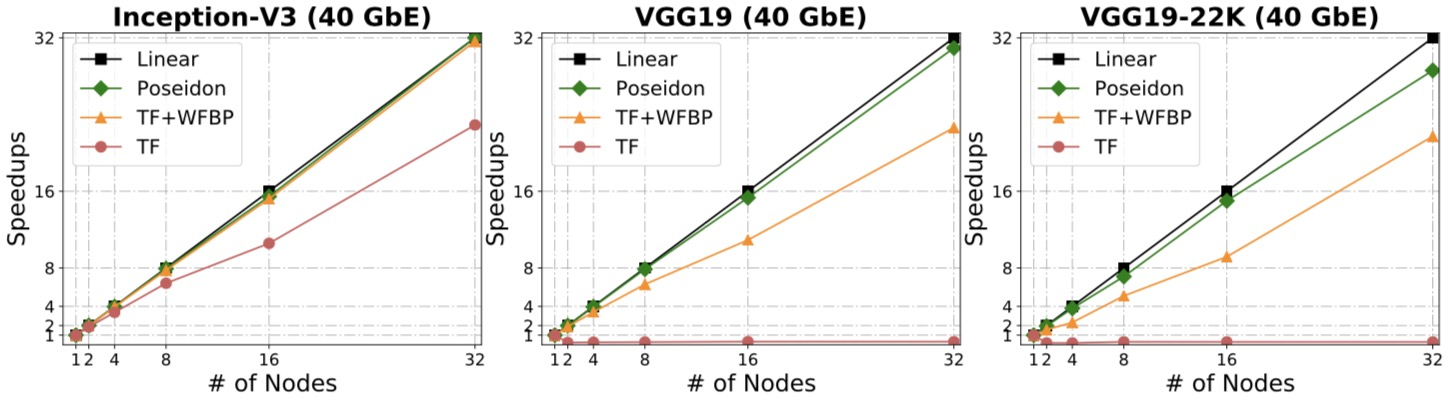
\includegraphics[width=14cm]{poseidon_result}
\caption{Poseidon实验对比图}
\label{fig:poseidon_result}
\end{figure}
由图~\ref{fig:poseidon_result}对比TF与TF+WFBP可知,WFBP算法对性能提升有巨大帮助,在参数量相对较小的网络(如inception-V3)中该算法即可保证网络达到近线性加速比。而在网络参数量较大,特别是全连接层参数量较大时,单使用WFBP算法不足以压缩同步参数的时间开销。因为全连接层计算量小而参数量大,使其对无法通过WFBP算法将通信延时隐藏在全连接层的反向计算中。而SFB算法正好解决了该问题。通过将全连接层M*N个参数分解成M+N个参数,极大减少了参数传输量。所以在全连接层占比较大的网络中,如VGG19,VGG19-22k等,加上SFB算法后分布式效率能接近理想加速比。

同年,Jianmin Chen等\upcite{bucketsgd2017}提出通过提供少量计算节点备份以缓解严格同步形成的木桶效应。论文首先通过大量实验验证了异步算法在神经网络训练中不能保证模型精度的问题,所以为保证训练精度应使用严格同步的优化算法。但是严格同步则导致每次迭代时间受计算最慢的机器的影响,随着集群增大,影响会越来越明显,为了避免这个影响,论文提出使用少量备份节点来减缓最慢机器导致的影响。假设集群中有53个计算节点同时计算,当server端接收到50个梯度后,就同步更新,剩下最慢的3个终止该次计算,这样能有效减少最慢的时间等待。这种通过备份节点来缓解木桶效应带来的影响具有非常好的启发意义。同时论文也提出下一步工作:用time-out,代替backup节点的想法要跟进。当80\%的梯度到达时,就更新参数,以这80\%的梯度代替所有的梯度进行更新。

同时,facebook等\upcite{train1hour2017}在Training ImageNet in 1 hour中提出两个简单且极为有效的调整学习率的方法:线性增大学习率和热启动方法。首先论文从sgd算法意义出发,从公式中推导出:当增大batch size时,线性增大学习率情况下,公式与原始batch size下的含义相同。同时在实际训练过程中,因为刚开始网络状态受初始化影响较大,且训练初期网络状态波动很大。学习率过大时,容易造成网络不收敛,故在训练刚开始阶段提出使用热启动的训练方法,从一个较小的学习率逐渐增长至线性增大策略所要求的学习率。实验结果如图~\ref{fig:training1hour_result}所示。

\begin{figure}[htp]
\centering
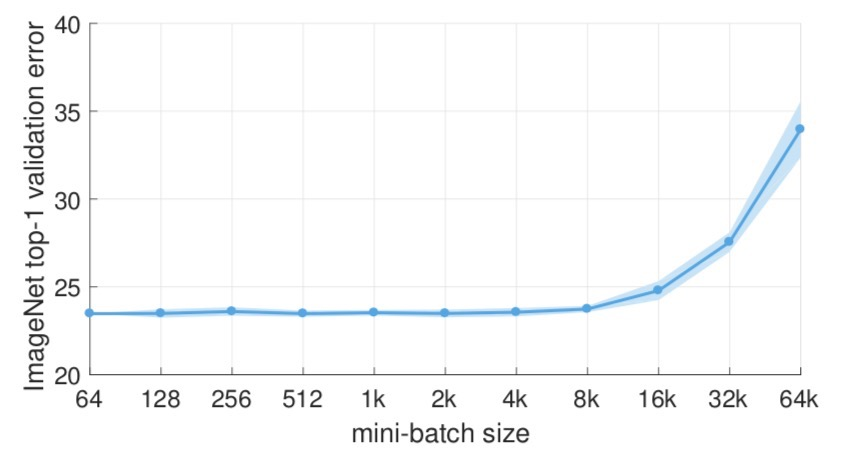
\includegraphics[width=12cm]{training1hour_result}
\caption{线性增大学习率和热启动方法下不同batch size下模型精度曲线}
\label{fig:training1hour_result}
\end{figure}
紧接着,伯克利尤洋等\upcite{train24min2017}提出分层自适应学习率算法。论文思想是不同网络层之间参数数值差距较大,而对应的梯度差距则更大,往往存在数量级之间的差距。作者指出不同网络层之间参数与梯度比值差距非常大,如果以相同的学习率来更新参数,必定造成较小参数更新步长过大,导致网络不收敛。故论文提出自适应各层参数大小的学习率调整方法,进一步将batch size由8k提升至32k,在24分钟内训完ImageNet。

随后,2018年Google Brain等\upcite{dontdecay2018}提出通过逐渐增大batch size替换学习率衰减的方法,最终将batch size提升至64k,只用两千五百多次迭代将ImageNet训到了理想精度。

\subsection{分布式深度学习中数据压缩的发展}
由2.1部分可知,分布式训练过程中同步通信量越小,分布式效率越高。近年来业界对在保证精度的情况下,如何尽可能地压缩传输梯度进行了相关研究。2017年,Xiangru Lian等\upcite{decentereasgd2017}提出去中心化的EASGD算法,减小网络通信量。在其环形拓扑结构中,每个worker只与其相邻的两个节点通信,将相邻两个节点的参数加和求平均,并求得本地参数与求得平均参数的差值更新至server。因为其更新的是参数的差值而不是参数本身,以此达到梯度压缩的目的。

2018年,Yujun Lin等\upcite{dgc2018}提出稀疏化梯度的方法。即每次只更新前0.1\%-1\%的梯度,极大减少了网络带宽,压缩比能达到600倍。剩下99.9\%未更新的梯度保留在本地,随着迭代的进行依次累加,直到该梯度达到前0.1\%~1\%后更新。


论文解释这种将梯度保留在本地的方法,类似于增大batch size。提出动量修正,梯度修剪,动量因子隐蔽,热启动等方法保证压缩后梯度的精度和延迟更新梯度的影响。其中动量修正示意图如图~\ref{fig:dgc_picture}所示。
\begin{figure}[htp]
\centering
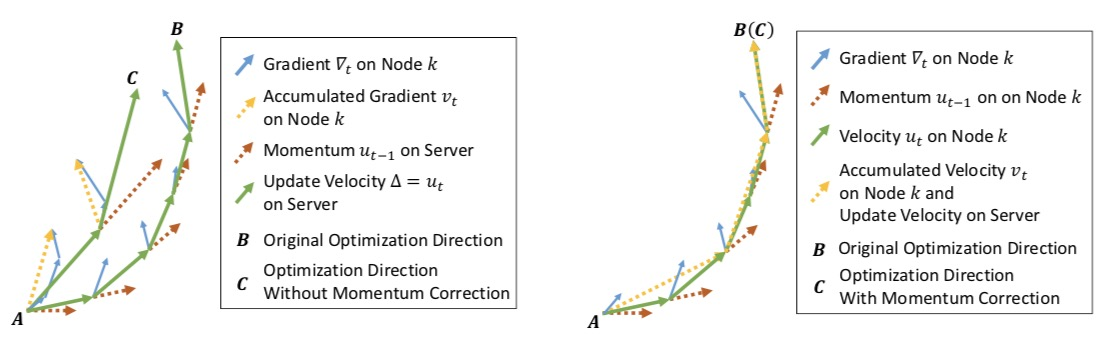
\includegraphics[width=14cm]{dgc_picture}
\caption{动量修正原理示意图}
\label{fig:dgc_picture}
\end{figure}

动量因子隐蔽灵感来源于Ioannis Mitliagkas\upcite{asynmomentum2016}论文中的implicit momentum思想,引入动量因子隐蔽,而不是搜索一个特定的动量(异步的程度越高,动量要设的越小),来减缓staleness。具体做法:只保留未更新梯度的动量因子,已更新梯度的动量因子置为0。如公式~\ref{equ:gdc_mask}所示。
\begin{equation}
\label{equ:gdc_mask}
\begin{split}
Mask\leftarrow |v_{k,t}|>thr \\
v_{k,t}\leftarrow v_{k,t}\odot ¬Mask \\
u_{k,t}\leftarrow u_{k,t}\odot¬Mask
\end{split}
\end{equation}

\section{本章小结}
本章主要介绍了分布式训练神经网络的特点,数据并行和模型并行这两种并行方法;介绍了神经网络在图像分类、物体检测、自然语言处理等领域的发展;最后详细介绍了分布式深度学习中涉及到的模型,系统,优化算法相关问题的研究进展。




